After a quick inspection of the dataset we understood that the data entries it contained were mostly complete but, at the same time, we didn't have enough information to infer the value of missing attributes for incomplete documents.

One useful thing that could have been done in the scenario of a real analysis would be to find another dataset containing technical data about single products, together with their ASIN, and use this information to compute a join over this attribute and complete our dataset with this additional data: anyway, while in the presented setting this information would be very easy to be retrieved, this was not our case, since we weren't able to find any additional dataset with these characteristics and we couldn't afford (both from resources and time perspective) to perform a snapshot of the Amazon website through scalping. 

The only interesting thing that is worth mentioning is the fact that we used a python script to extract a subset of the dataset:\\
\begin{lstlisting}[language=Python]
import os

os.chdir("../Datasets")
json_file_path = os.path.join(os.getcwd(), "Digital_Music.json")
n = 150_000
suffix = str(n//1000) + "k"
output_file_path = json_file_path[:-5] + "_" + suffix + ".json"

with open(json_file_path, 'r') as input_file:
    with open(output_file_path, 'w') as output_file:
        for i in range(n):
            # EACH OBJECT MUST OCCUPY *EXACTLY* ONE LINE
            output_file.write(input_file.readline())
\end{lstlisting}

Specifically, as it can be seen, we used this script to round the number of documents to the nearest multiple of 50.000 by extracting the first lines of the original file.
It is worth noticing that the core lines of this script can be easily modified to perform any kind of filtering over the JSON documents in this way:\\
\begin{lstlisting}[language=Python]
import os
import json

os.chdir("../Datasets")
json_file_path = os.path.join(os.getcwd(), "Digital_Music.json")
n = 150_000
suffix = str(n//1000) + "k"
output_file_path = json_file_path[:-5] + "_" + suffix + ".json"

with open(json_file_path, 'r') as input_file:
    with open(output_file_path, 'w') as output_file:
        i = 1
        while i <= n:
            # EACH OBJECT MUST OCCUPY *EXACTLY* ONE LINE
            line = input_file.readline()

            # Be sure that the line is not empty
            if not line:
                break
                
            json_object = json.loads(line)

            # Generic filter
            if filter:
                output_file.write(line)
                i += 1
\end{lstlisting}
Anyway we decided to not apply any further filtering since we wanted to keep as many attributes as possible in order to be more free in the writing of the queries and eventually realize these filters through them: just keep in mind that, with larger data collections, it could be more efficient to perform filtering beforehand (e.g. to consider only reviews published from a specific point in time on) and this could be a way of doing it.

\begin{figure}[H]
    \centering
    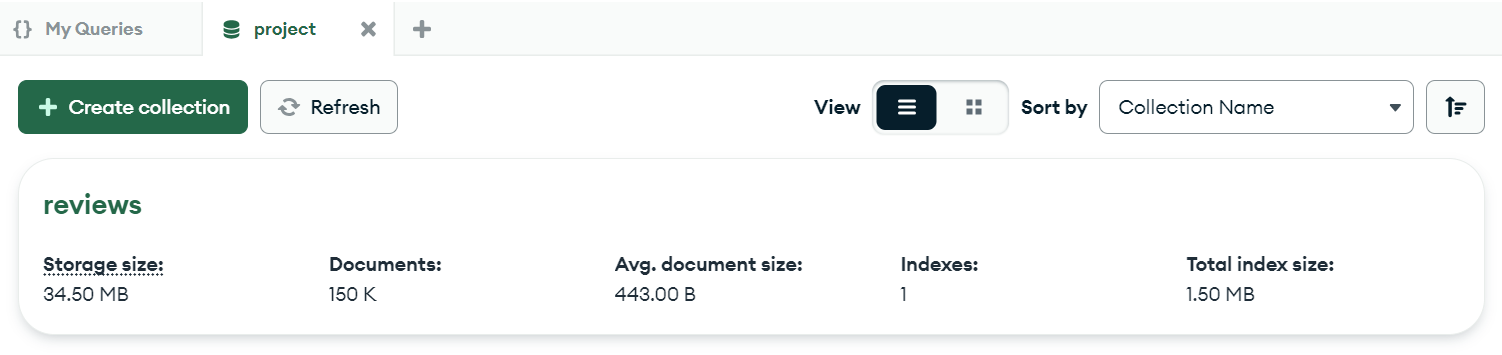
\includegraphics[scale=0.4]{Images/db_occupation.png}
    \caption{Physical occupation of the database on disk}
\end{figure}